\documentclass{article}
\usepackage{amsmath}
\usepackage{MnSymbol}
\usepackage{wasysym}
\usepackage{graphicx}
\usepackage{listings}

\begin{document}
\begin{center}
\LARGE \bfseries{Answers to Problem Set 1}\\
 Group name: Ferienspass\vspace{.5cm}\\
 \normalsize \normalfont
  Sebastian K\"uhnl: 5642348\\
  Alexander D\"uck (as: reebyte): 5504077\\
  Patrick Blank (as: paddyblank): 6729110\\
  Christian Wierschem: 6729288
\end{center}
\normalsize	

\section{Question 1}

\subsection{}
A market equilibrium occurs when markets clear. This implies no excess demand ($D$) or supply ($S$) of Goods. Thus, $q_D = q_S$. This only occurs when $p_D = p_S$ (the market clearing price prevails).
\begin{center} $p_D = p_S$ \end{center}
using
\begin{center} $p_D=a-b*q_D $ and $p_S=c+d*q_S$\end{center}
 we get
\begin{center} $a-b*q_D =c+d*q_S$ \end{center}
\begin{center} $0 =c+d*q_S-(a-b*q_D)$ \end{center}
\begin{center} $0 =c-a+d*q_S+b*q_D$ \end{center}
\begin{center} $0 =b*q_D+d*q_S-(a-c)$ \end{center}
Since $q_D = q_S$ holds, this can be simplified even further 
 \begin{equation} \label{First_One}0 =(b+d)*q-(a-c)\end{equation} $\blacksquare$
 
\subsection{}

Analytical computation of the equilibrium allocation. Alternative approach of previous question used. First, set quantities equal, $q_D = q_S$ and calculate the resulting equilibrium price $p^{*}$. By inserting the equilibrium price into both quantity functions, we get the equilibrium quantity and can show that $q_D = q_S$ in fact holds.
\begin{center} $q_D = q_S $ \end{center}
\begin{center}$\frac{a-p}{b} = \frac{c-p}{d} $ \end{center}
\begin{center}$d(a-p) = b(p-c)$ \end{center}
\begin{center}$da+bc=p(d+b)$ \end{center}
\begin{center}$\frac{da+bc}{d+b} = p^{*}$\end{center}
Now, insert into the quantity functions:
\begin{center} \begin{tabular}{ l l }
   $q_D= \frac{a-p^{*}}{b} $ & $q_S= \frac{c-p^{*}}{d} $  \\
   & \\
   $q_D= \frac{a-\frac{da+bc}{d+b}}{b} $ & $q_S= \frac{c-\frac{da+bc}{d+b}}{d} $  \\
   & \\
   $q_D= \frac{a-c}{d+b}=q $ & $q_S= \frac{a-c}{d+b}=q $  \\ \end{tabular} \end{center}
which can also be computed by rearranging \eqref{First_One}:
\begin{center}$0 =(b+d)*q-(a-c)$ \end{center}
\begin{center}$(a-c) =(b+d)*q$ \end{center}
\begin{center}$\frac{a-c}{b+d}=q$ \end{center}

\subsection{}
The LU decomposition. The application of this procedure can be found in the MATLAB file PS1Q1.m.\\
\begin{enumerate}
\item Rearrange the equations given in the problem set so that, when solving for x, we solve for $x = [p, q]'$.
\begin{center}$a= p+bq $ \end{center} \begin{center}$ c=p-dq$ \end{center}
Which gives the system

\begin{center}$ \begin{pmatrix}
  1 & b  \\
  1 & -d 
 \end{pmatrix}
 \begin{pmatrix}
  p \\
  q 
 \end{pmatrix}
 =
  \begin{pmatrix}
  a \\
  c 
 \end{pmatrix}$\end{center}

\item Decompose the matrix A into the two factors L and U:
\begin{center} $ A= L*U=
 \begin{pmatrix}
  1 & 0 \\
  1 & 1
 \end{pmatrix}
  \begin{pmatrix}
  1 & b \\
  0 & -b-d
 \end{pmatrix} $ \end{center}
Which then gives the following system of equations:
\begin{center}$ \begin{pmatrix}
  1 & 0 \\
  1 & 1
 \end{pmatrix}
  \begin{pmatrix}
  1 & b \\
  0 & -b-d
 \end{pmatrix}
 \begin{pmatrix}
  p \\
  q 
 \end{pmatrix}
 =
  \begin{pmatrix}
  a \\
  c 
 \end{pmatrix}$\end{center}
\item Solve this system of equations.
\begin{enumerate}
\item First solve $Ly=b$ by forward induction.
 \begin{center} $\begin{pmatrix}
  1 & 0 \\
  1 & 1
 \end{pmatrix}
 \begin{pmatrix}
  y_1 \\
  y_2
 \end{pmatrix}
 =
  \begin{pmatrix}
  a \\
  c
 \end{pmatrix} $ \end{center}
 \begin{center} $  y_1=a$  \end{center}
 \begin{center} $y_1+y_2=c $ \end{center}
which gives
 \begin{center} $  y_1=a$  \end{center}
 \begin{center} $y_2=c-a$ \end{center}
\item Then solve $Ux=y$ by backward induction.
 \begin{center} $\begin{pmatrix}
  1 & b \\
  0 & -(b+d)
 \end{pmatrix}
 \begin{pmatrix}
  p \\
  q
 \end{pmatrix}
 =
   \begin{pmatrix}
  y_1 \\
  y_2
 \end{pmatrix}
 =
  \begin{pmatrix}
  a \\
  c-a
 \end{pmatrix}$ \end{center}
 \begin{center}$ -(b+d)q=y_2=c-a $ \end{center}
 \begin{center}$p+b q=a $ \end{center}
which gives
 \begin{center}$ q=\frac{a-c}{b+d} $ \end{center}
 \begin{center}$ p = \frac{ad+bc}{b+d} $ \end{center}
\end{enumerate}
\end{enumerate}

\newpage
\subsection{}

\lstinputlisting[linerange={1-20}]{PS1Q1.m}
LU Result: The market clearing price 2.3333 clears the market at the quantity 1.3333!


\subsection{}

\paragraph{Convergent case}

\lstinputlisting[linerange={21-32, 42-76}]{PS1Q1.m}
Gauss-Seidel Iteration Result (using quantity as initial guess): The market clearing price 2.3357 clears the market at the quantity 1.3357 after 9 iterations!\\[2em]

\lstinputlisting[linerange={78-117}]{PS1Q1.m}
Gauss-Seidel Iteration Result (using price as initial guess): The market clearing price 2.3312 clears the market at the quantity 1.3312 after 11 iterations!\\[2em]

\lstinputlisting[linerange={119-167}]{PS1Q1.m}
\begin{figure}[h!]
\centering
    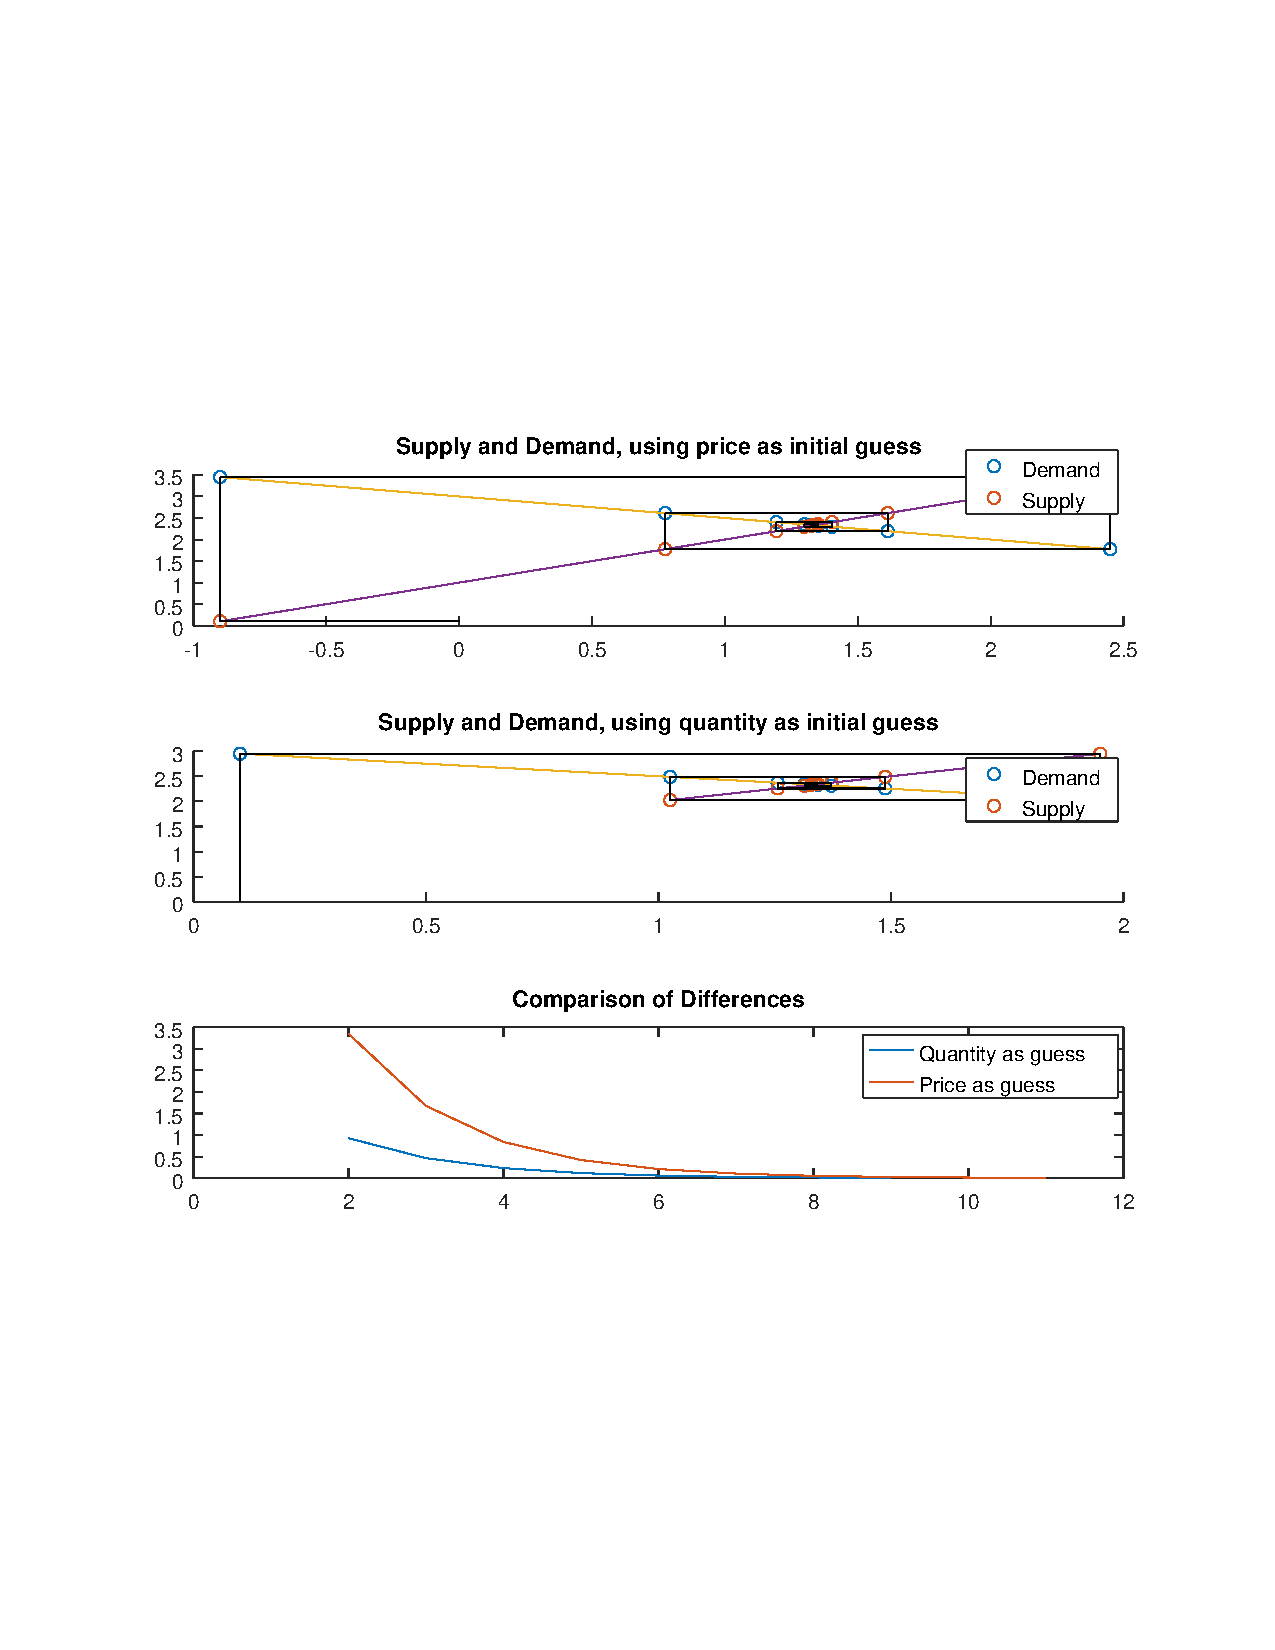
\includegraphics[width=0.99\textwidth]{figure1}
\end{figure}

\paragraph{Non-convergent case}

\lstinputlisting[linerange={169-177, 187-235}]{PS1Q1.m}
\begin{figure}[h!]
\centering
    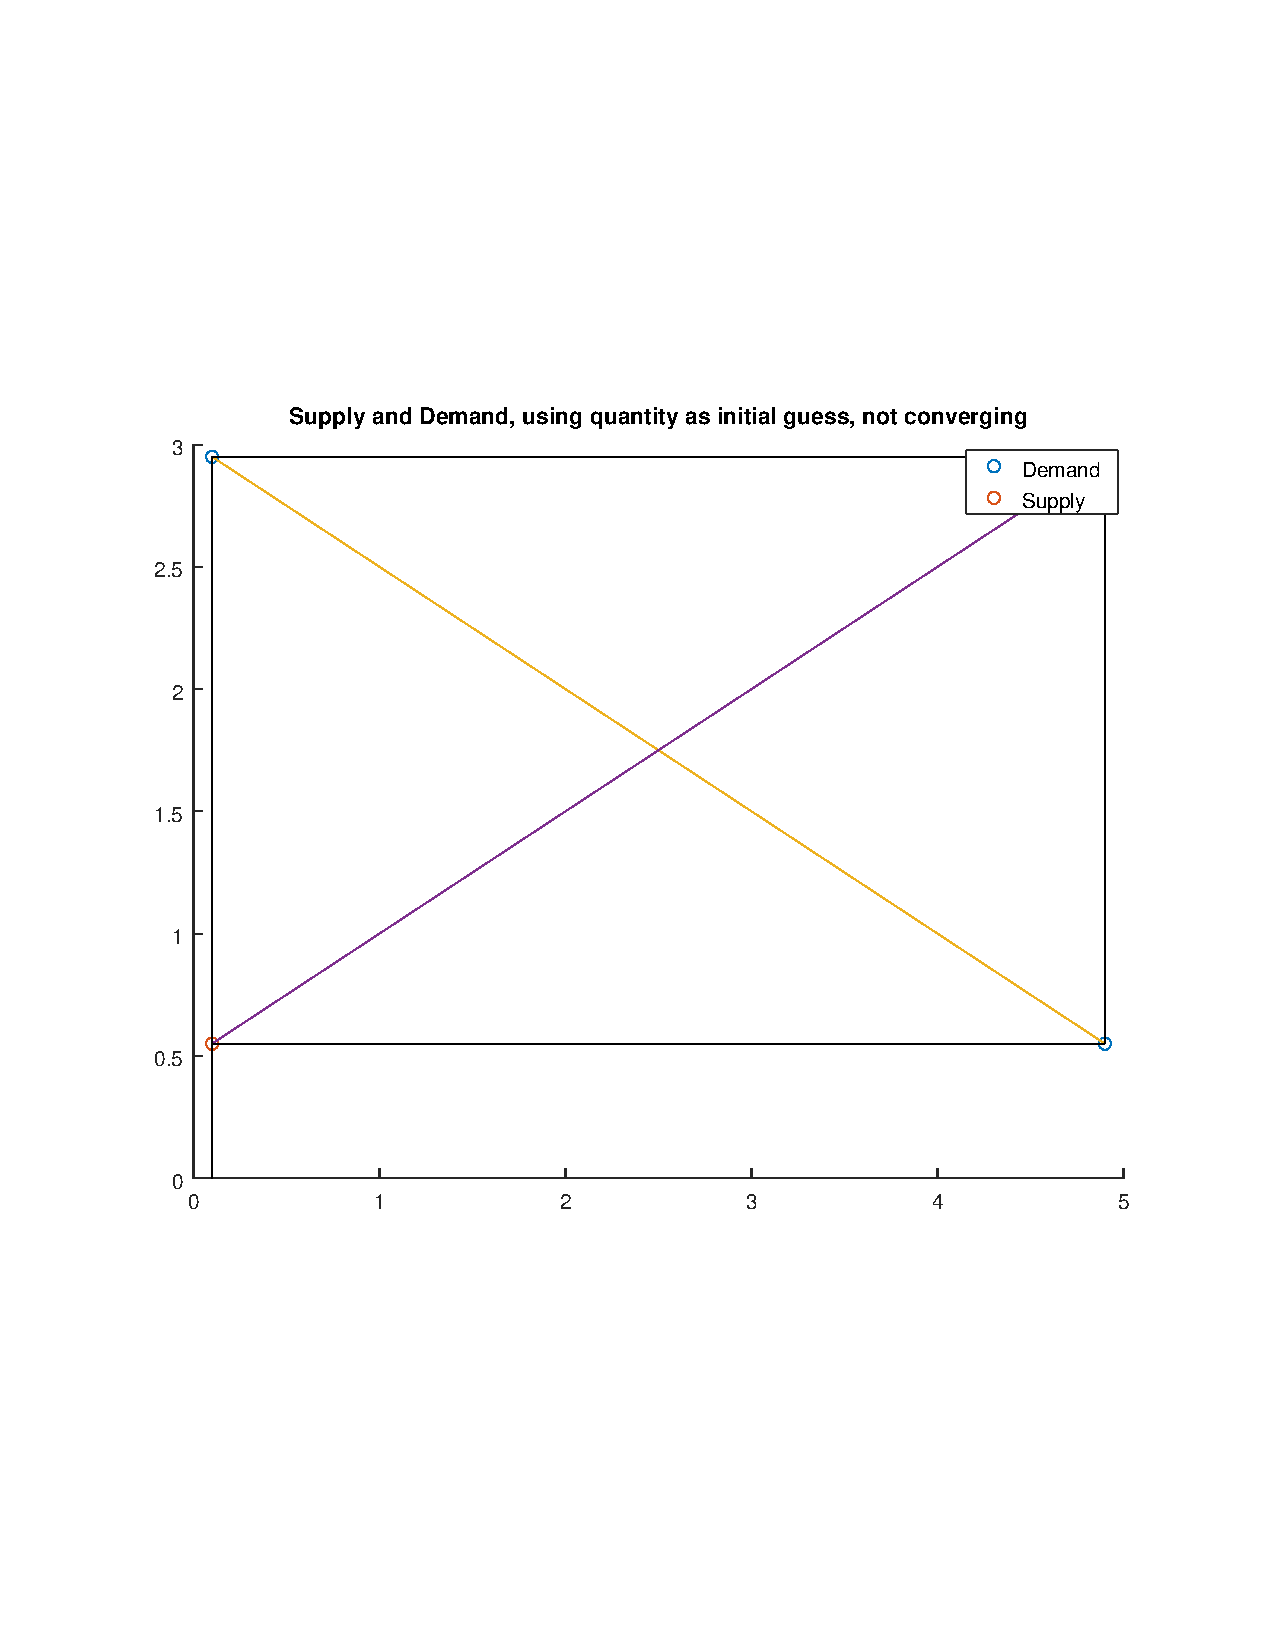
\includegraphics[width=0.8\textwidth]{figure2}
\end{figure}


\subsection{}
\lstinputlisting[linerange={238-311}]{PS1Q1.m}
\begin{figure}[h!]
\centering
    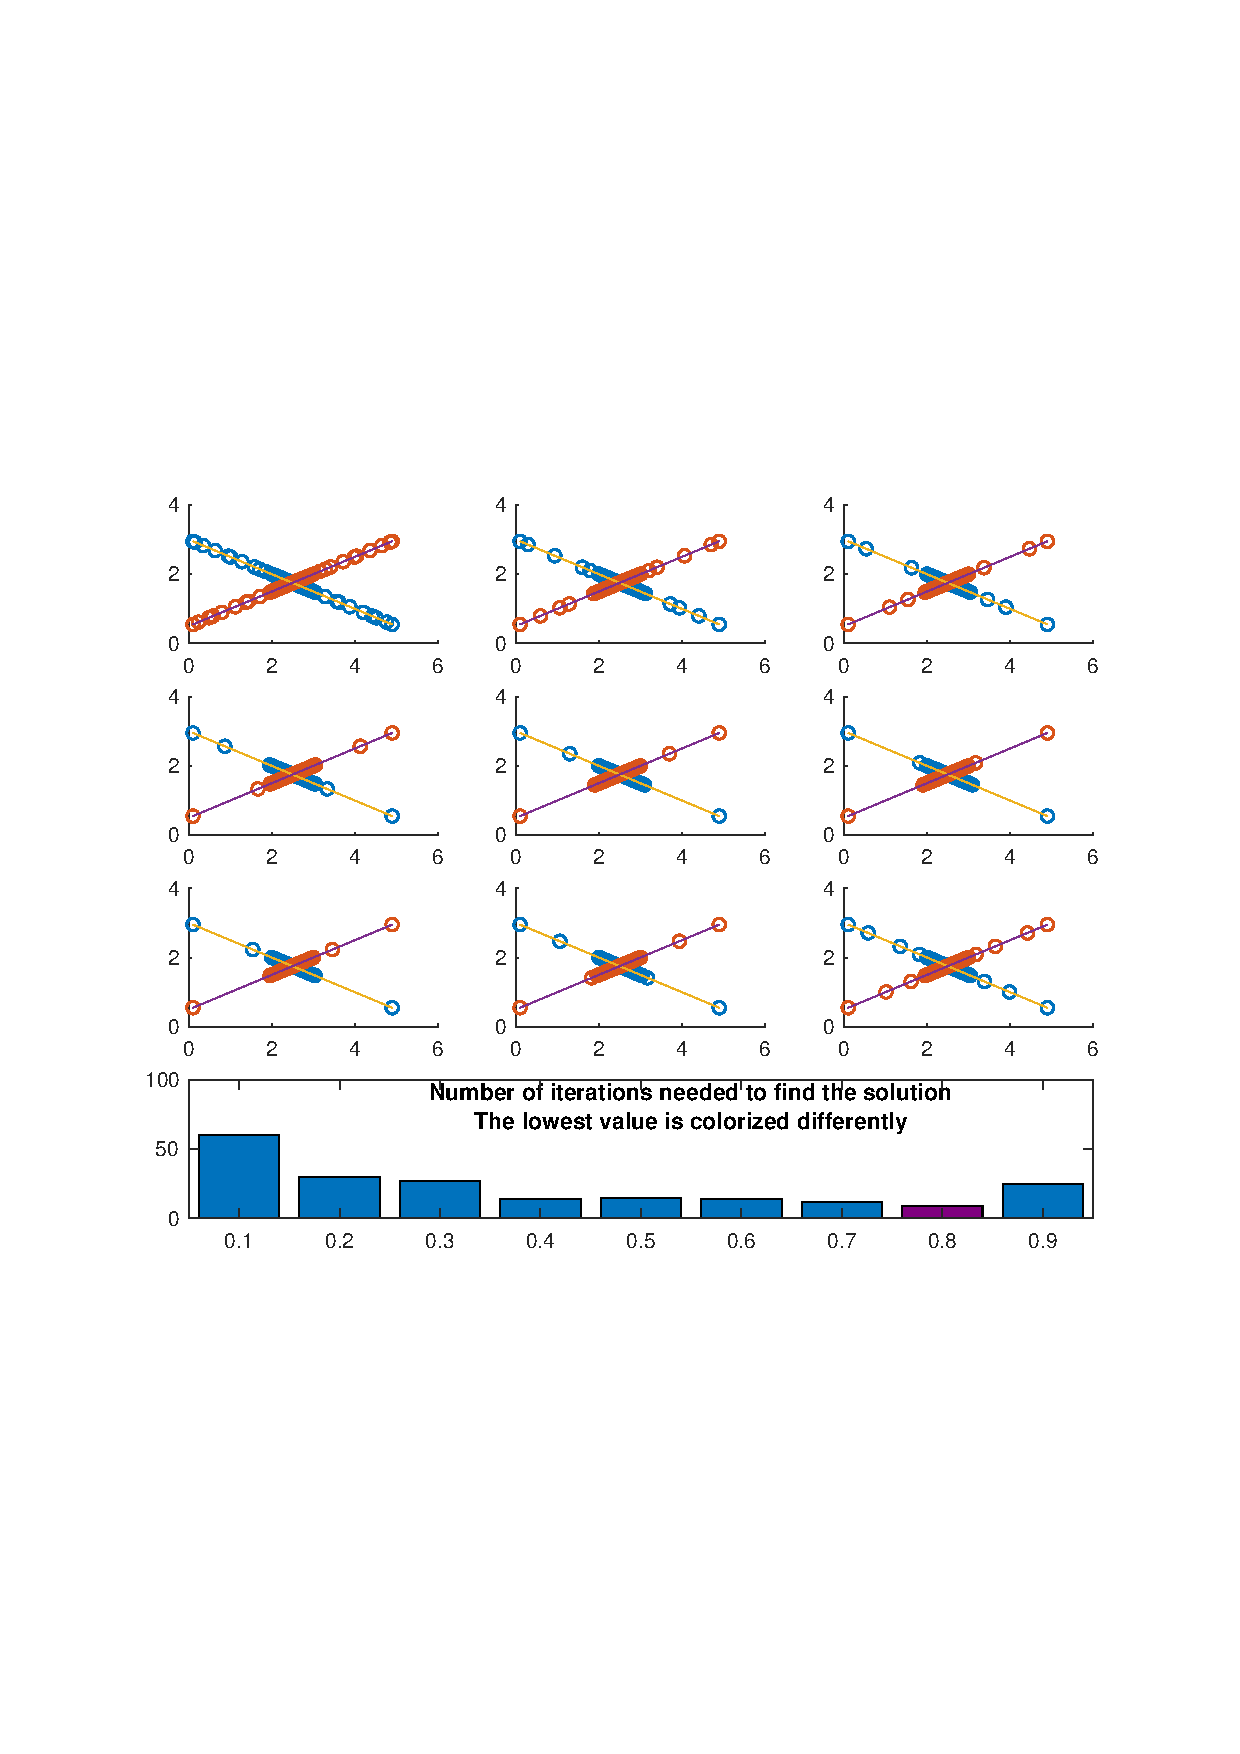
\includegraphics[width=0.99\textwidth]{figure3}
\end{figure}

\newpage
\section{Question 2}

\subsection{}
\lstinputlisting[linerange={1-10}]{P1Q2.m}

\subsection{}
\lstinputlisting[linerange={12-17}]{P1Q2.m}

\subsection{}
\lstinputlisting[linerange={19-27, 28-46}]{P1Q2.m}

\subsection{}
\lstinputlisting[linerange={53-65}]{P1Q2.m}

\subsection{}
\lstinputlisting[linerange={67-76}]{P1Q2.m}
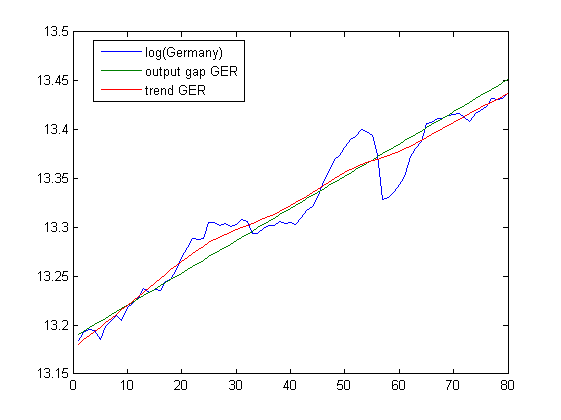
\includegraphics[width=0.99\textwidth]{plot1.png}\\
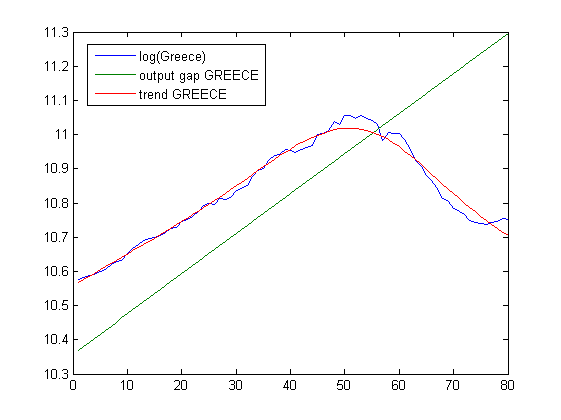
\includegraphics[width=0.99\textwidth]{plot2.png}\\
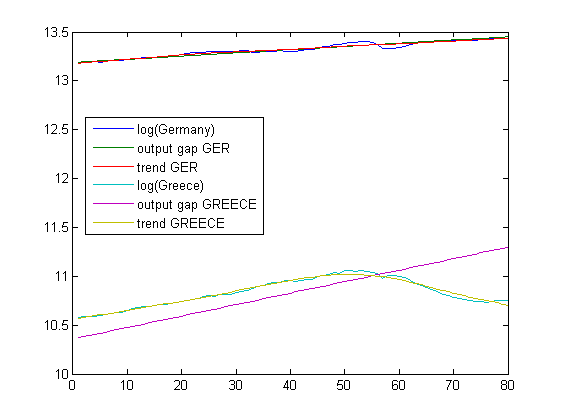
\includegraphics[width=0.99\textwidth]{plot3.png}
\newpage
\section{Question 3}

\begin{figure}[h!]
\centering
    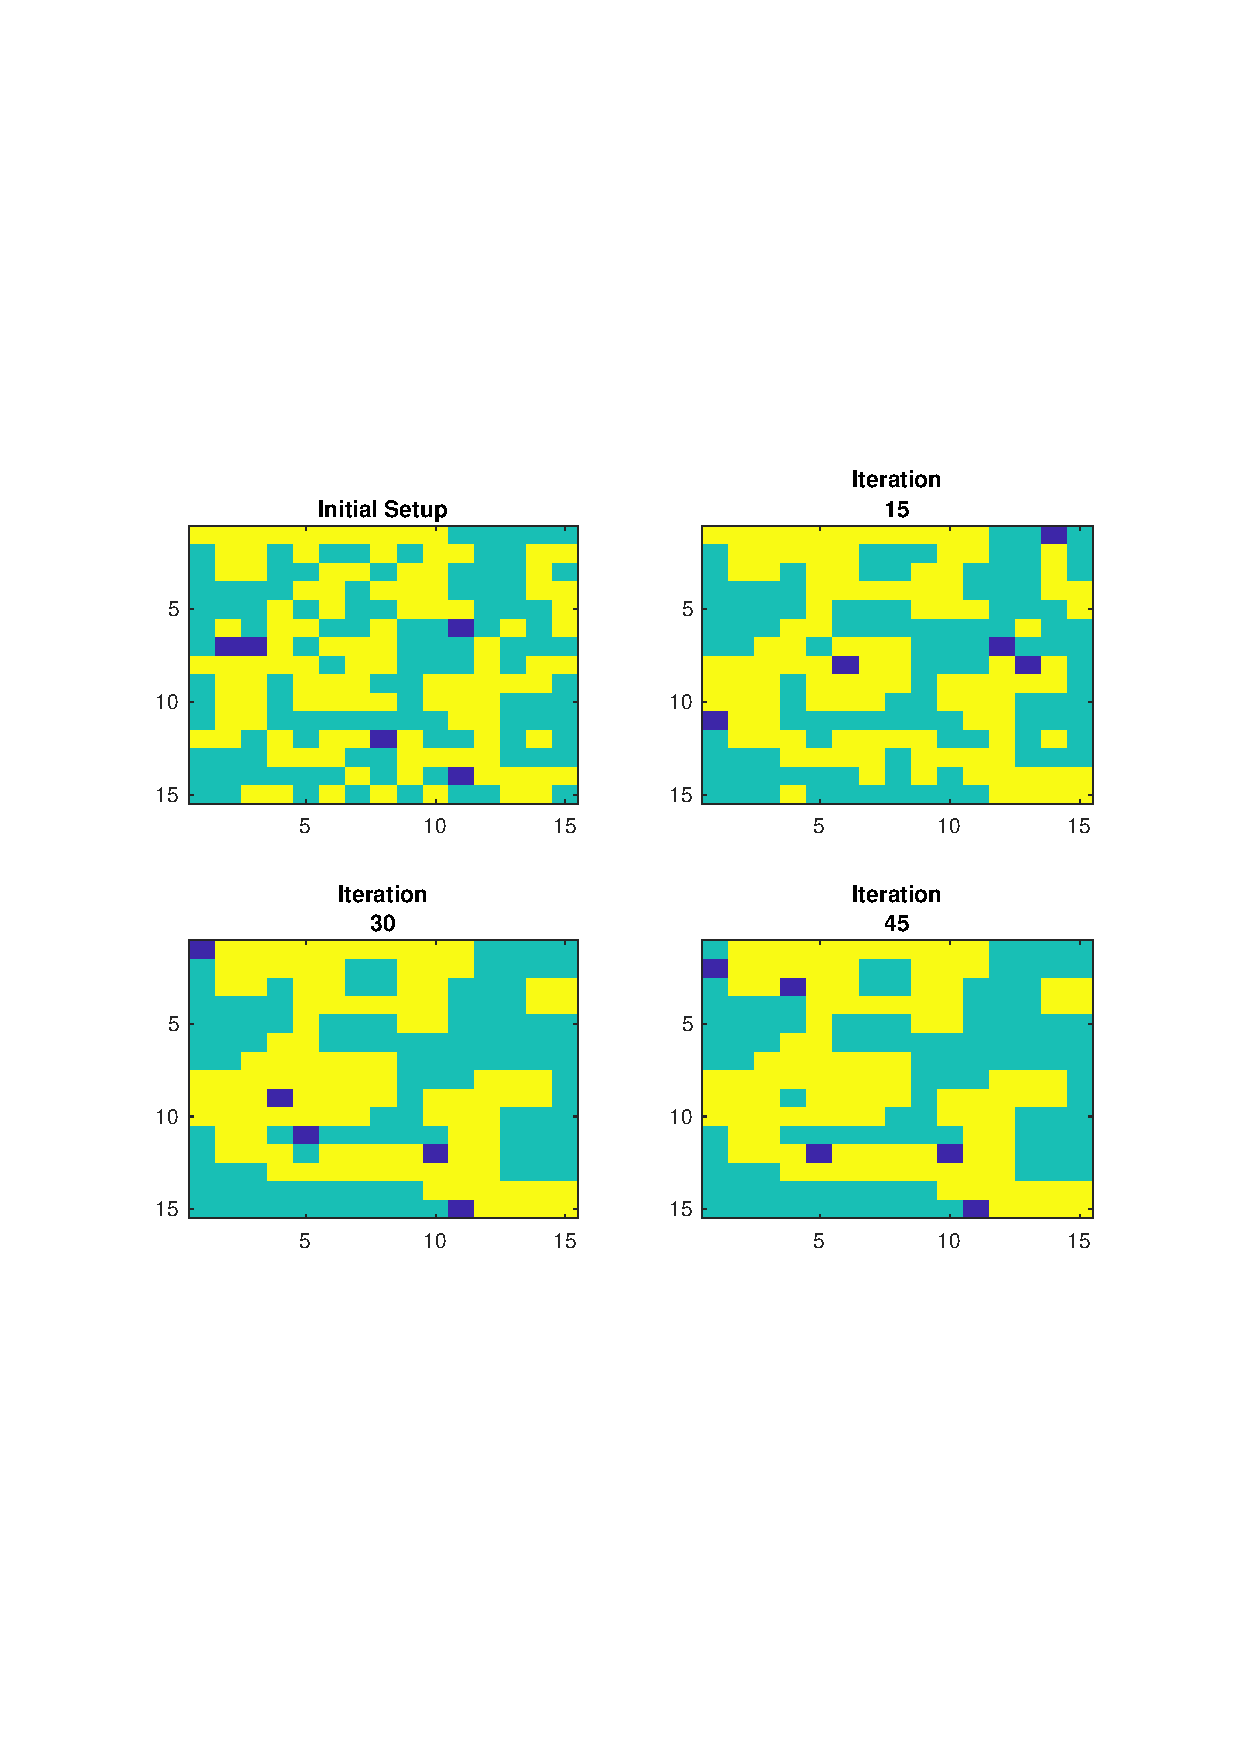
\includegraphics[width=0.99\textwidth]{figure_schelling}
\end{figure}
\lstinputlisting{PS1Q3.m}
\appendix
	\section{Alternative Moving Understanding P3}
\lstinputlisting{MyPS1P3.m}	
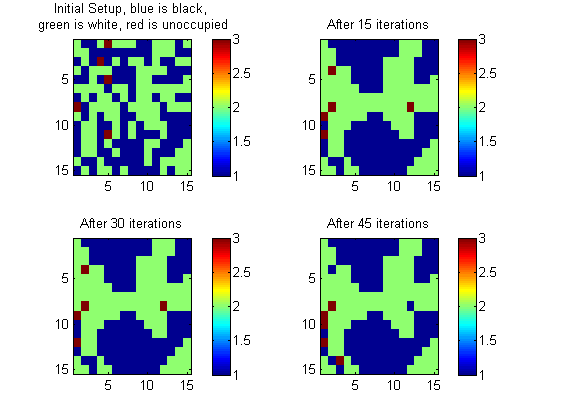
\includegraphics[width=0.99\textwidth]{Moving.png}
\end{document}